% ||================================================================================================
% || Präambel
% ||================================================================================================

% |=================================================================================================
% | Layout
% |=================================================================================================
\documentclass[12pt,titlepage]{report}
% digital
% print
%\documentclass[12pt,titlepage]{book}
\usepackage{geometry}
\geometry{
  left=3cm,
  right=3cm,
  % print
  % bindingoffset=5mm
}

% |=================================================================================================
% | Fonts
% |=================================================================================================
\usepackage[onehalfspacing]{setspace}
\usepackage{dejavu} 
\usepackage{sectsty}
\allsectionsfont{\sffamily}
\usepackage[T1]{fontenc}
\usepackage[utf8]{inputenc} % direkte Einbgabe von Umlauten

% language stuff
\usepackage[german]{babel}

% miscellaneous
\usepackage{graphicx, subfigure}         % graphics
\graphicspath{{grafiken/}}
\usepackage[german]{fancyref}
\usepackage{hhline}           % double lines in tables
\usepackage{amsfonts}         % real numbers etc.
\usepackage[rightcaption]{sidecap} % figure captions on the right (optional)
\usepackage{hyperref}         % for URLs
\usepackage{listings}         % for code samples
\usepackage{fancyhdr}         % for header line

\usepackage[backend=biber, style=authoryear-icomp]{biblatex}
\addbibresource{literatur.bib}
% \usepackage{natbib}
% Hier bei Bedarf die Seitenränder einstellen
\usepackage[german]{algorithm2e}
\RestyleAlgo{ruled}

\usepackage[german]{cleveref}

\usepackage[printonlyused]{acronym}
\usepackage{multirow, multicol, tabularx}
\usepackage{csquotes}
\newcommand*{\fancyrefalgolabelprefix}{algo}

\newcommand*{\Frefalgoname}{ALGORITHMUS}
\newcommand*{\frefalgoname}{Algorithmus}

\frefformat{plain}{\fancyrefalgolabelprefix}{\frefalgoname\fancyrefdefaultspacing#1}
\Frefformat{plain}{\fancyrefalgolabelprefix}{\Frefalgoname\fancyrefdefaultspacing#1}

\frefformat{vario}{\fancyrefalgolabelprefix}{\frefalgoname\fancyrefdefaultspacing#1#3}
\Frefformat{vario}{\fancyrefalgolabelprefix}{\Frefalgoname\fancyrefdefaultspacing#1#3}

% Kopf- und Fußzeile
\fancyhead{} % clear all header fields
%\fancyhead[RO,LE]{\leftmark}
\fancyhead[RO]{\leftmark}
\setlength{\headheight}{15pt}

\title{Arbeit}
\author{Alexander Martin}
\date{August 2021}

\begin{document}

\begin{titlepage}
  \begin{center}
    {\Large\bf Entwurf und Implementierung einer generischen Ingestion-Schnittstelle mit Versionierung für Data-Lake-Systeme}\\[2cm]

    {\bf Masterarbeit}\\
    zur Erlangung des Grades {\em Master of Science}\\[1cm]

    an der\\
    Hochschule Niederrhein\\
    Fachbereich Elektrotechnik und Informatik\\
    Studiengang {\em Informatik}\\[2cm]

    vorgelegt von\\
    Alexander Martin\\
    1018332\\[3cm]
    Datum: \today\\[2cm]

    Prüfer: Prof.~Dr.~rer.~nat.~Christoph Quix\\
    Zweitprüfer: Sayed Hoseini,~M.Sc.

  \end{center}
\end{titlepage}
\newpage
\include{unabhänhigkeit}
\newpage
\section*{Zusammenfassung}

Heutzutage spielen Daten eine immer wichtiger Rolle.
Durch den vermehrten Einsatz von IoT-Geräten und moderne Cloud-Speicher-Lösungen, wächst die Zahl an anfallenden Daten vielen Firmen und Forschungseinrichtungen stetig.
Mit steigenden Datenmengen und der diversen Strukturen der Daten ist deren Verwaltung ein komplexes Thema geworden.
Diese Arbeit befasst sich mit der technischen Herausforderung Daten aus verschiedensten Quellen zu Verwalten.
Als Lösung hierfür wurden Data-Lake-Systeme vorgeschlagen.
Im Kontext des HIT-Institut der Hochschule Niederrhein, wurde ein Prototyp für einen Data-Lake entwickelt.
In dieser Arbeit wird eine Schnittstelle entwickelt, über die Benutzer Daten aus unterschiedlichen Quellen in dieses System laden können.
Dabei werden Metadaten über die Datenquellen gesammelt.
Mit der Schnittstelle ist es auch möglich, die geladenen Daten zu versionieren, um weiter Verarbeitungen effizienter zu machen.

\section*{Abstract}

In todays world data play an important role.
The amount of data in comapnies and research facilities is growing due to the increasing use of IoT-devices and modern Cloud-Storage-Solutions.
With the bigger amount of data and their varying structures the data management got more complex.
This thesis takes on the technical challenge of managing data from different sources.
Data lakes are a proposed solution for this problem.
A prototype for a data lake was developed at the HIT-institute at the Hochschule Niederrhein.
This thesis devolopes an interface for users to ingest data from diffenrent sources to the system.
The interface collects metadata about the data sources.
It is also capable of saving data with versioning to make further processing more efficient.
\newpage

\pagestyle{fancy}
\tableofcontents
\newpage

\chapter{Einleitung}

Heutzutage spielen Daten eine immer wichtiger Rolle.
In vielen Firmen und Forschungseinrichtungen wächst die Zahl an unterschiedlichen Daten stetig.
Im \textit{Rethink Data Report 2020} \textcite{rethink_data_2020} wurde eine Studie durchgeführt, die eine Steigerung von 42\% der Menge an anfallenden Daten pro Jahr prognostiziert.
Diese Daten sind zum Beispiel durch den vermehrten Einsatz von IoT-Geräten oder ausführlicher werdende Analysen zurückzuführen.
Auch, dass es durch moderne Cloud-Speicher-Lösungen einfacher geworden ist große Datenmengen zu speichern, begünstigt diese Entwicklung.
Daten sind eine wertvolle Ressource und müssen entsprechend gut verwaltet werden.
Durch die unterschiedlichen Formate und Strukturen, zum Beispiel Datenbanktabellen, JSON-Datei oder Bilder ist die Verwaltung ein komplexes Thema.
Die Bewältigung der organisatorischen Aufgaben fällt in den Bereich Data Governance.
Diese Arbeit beschäftigt sich mit den technischen Herausforderungen Daten aus einer Vielzahl von Datenquellen zu verwalten.

In vielen Unternehmen besteht das Problem, dass Daten in sogenannten Datensilos gelagert werden.
Das bedeutet, dass für verschiedene Anwendungen oder Format isolierte Speichersysteme verwendet werden.
Dabei entsteht das Problem, dass der Überblick, welche Daten es in der gesamten Systemlandschaft gibt verloren geht.
Auch Daten, für Analysen, untereinander zu Verknüpfen wird mit zunehmender Datenmenge und Variation schwieriger.

Ein klassischer Ansatz, der die Analysen vereinfachen soll ist das Data Warehouse.
Ein Data Warehouse besteht aus verschiedenen Datamarts, in denen Daten für bestimmte Analysen abgelegt werden.
Daten werden aus den Quellsystemen geladen, mit verschiedenen Transformationen auf ein für den Datamart globales Schema gebracht und dann abgespeichert \parencite{dw}.
Dieses Vorgehen wird auch ETL (Extract Transform Load) genannt, da die Daten erst aus der Quelle extrahiert, dann transformiert und gespeichert werden und erst nach diesen Schritten für eine Analyse geladen werden können.
Bei der Transformation der Daten kann es oft passieren, dass ein Teil ihres Informationsgehalts verloren geht, da nicht alle Felder in den Datamart übernommen werden.
Außerdem wird eine Änderung an einem Schema teurer, je mehr Daten bereits integriert wurden.
Als Lösung für diese Problem wurden Data Lakes vorgeschlagen \parencite{dixon2010pentaho,datalake_03}.

\section{Data-Lake-Systeme}
\label{sec:einleitung-datalake}

Ein Data Lake ist ein System, das die Erfassung, Verfeinerung, Archivierung und Erkundung von Daten vereinfacht und verbessert \parencite{datalake_01}.
Es sollen große Datenmengen möglichst kostensparend speichern und verschiedenste Formate verarbeiten werden können \parencite{datalake_02}.
Diese System verfolgen dabei den ELT (Extract Load Transform) Ansatz.
Das Kernprinzip ist die Speicherung der Daten in ihrem Rohformat.
Die Transformation findet erst statt, nachdem die Daten für weitere Verarbeitungen geladen wurden.
Dadurch fällt der Aufwand für eine Transformation vor dem Speichern, wie bei einem Data Warehouse, weg und Daten sind schneller für weitere Verarbeitungen bereit.
Außerdem gehen dabei keine Informationen mehr verloren.

Ein Data-Lake-System basiert auf vier verschiedenen Ebenen, wie zum Beispiel in \cref{fig:datalake}.
Diese sind die Interaktion-, Transformations-, Speicher- und Ingestion-Ebene.
Über die Interaktions-Ebene kann auf die Daten im Data Lake zugegriffen und Metadaten verwaltet werden.
Die Transformations-Eben bereitet die Daten auf, nachdem diese aus der Speicher-Ebene geladen wurden.
Als letztes gibt es die Ingestion-Ebene.
Diese ist für die Integration von Daten in den Data Lake verantwortlich.
Gleichzeitig werden hier auch Metadaten aus den Daten extrahiert.
Die Umsetzung eines solchen Data  Lakes kann je nach Voraussetzungen des Einsatzbereichs variieren.

\begin{figure}
    \centering
    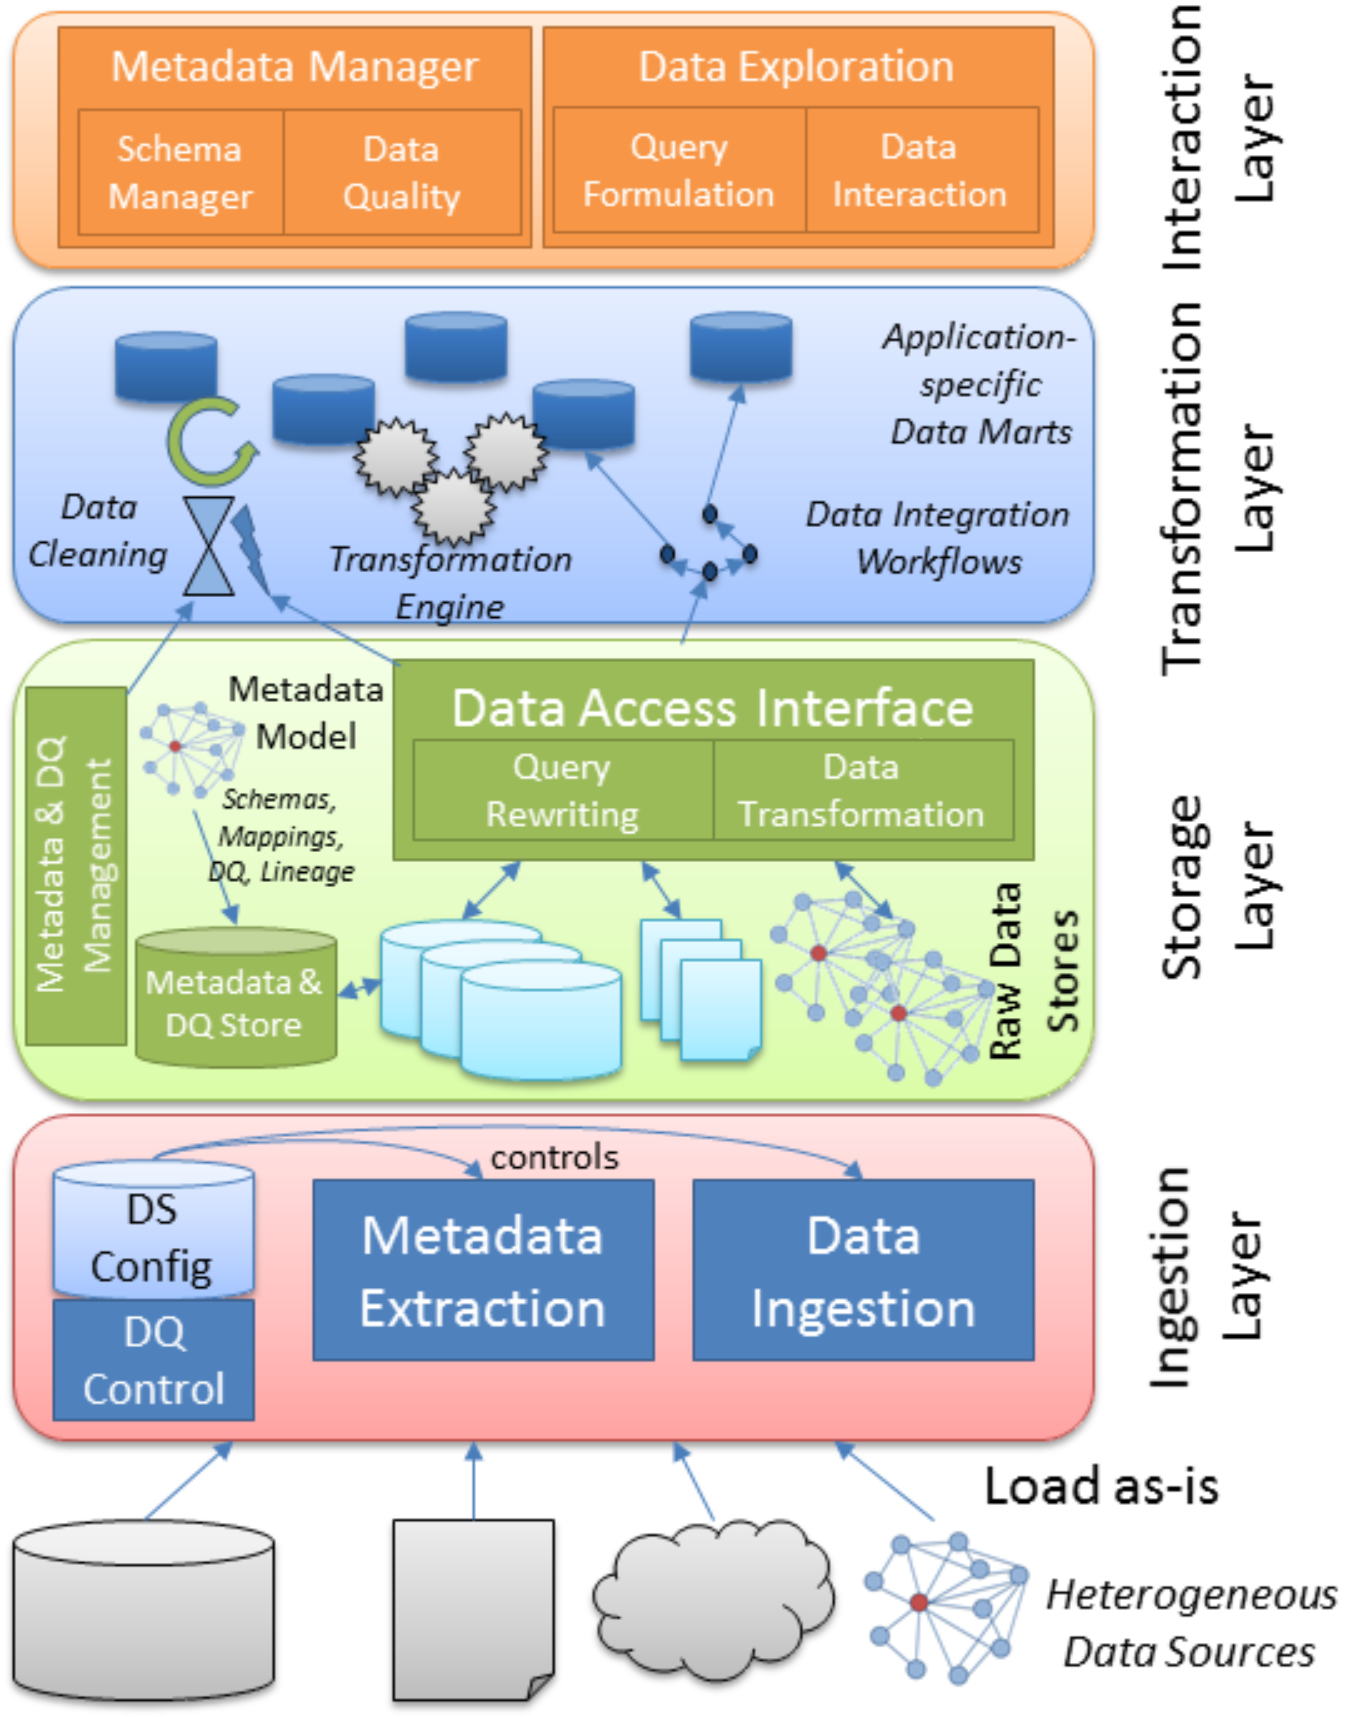
\includegraphics[width=.645\textwidth]{Grafiken/data_lake_architecture.PNG}
    \caption{Architektur eines Data Lakes \parencite{datalake_03}}
    \label{fig:datalake}
\end{figure}
\vfill

\pagebreak

\section{Motivation}
\label{sec:einleitung-motivation}

In einem Data Lake spielen die Metadaten eine zentrale Rolle.
Die Qualität der Metadaten bestimmt, wie gut Daten im Data Lake gefunden und in einen Zusammenhang gebracht werden können.
In den Metadaten können dabei sowohl Informationen über die Herkunft von Daten als auch über deren Inhalt oder Qualität stehen.

Für das HIT-Institut der Hochschule Niederrhein soll ein Data Lake entwickelt werden, der für die Verwaltung der Daten eingesetzt wird.
In diesem System sollen verschiedene Quellen zusammengebracht werden.
Dazu gehören Datenbank-Systeme, Dateien und Daten aus speziellen Software-Systemen, die über eine REST-API erreichbar sind.
Hier sollen die Daten jedoch nicht nur einmalig in das System geladen, sondern kontinuierlich aktualisiert werden.
Der einfachste Ansatz ständig den vollständigen Datensatz hinzuzufügen ist jedoch zu aufwändig und speicherintensiv.
Daher muss das Data-Lake-System eine Versionierung der Daten unterstützen und Änderungen in den Quellen erkennen können, so dass nur diese gespeichert werden.
Dies würde auch weiteren Prozessen, wie Transformation, Integration oder Analyse der Daten beschleunigen.
Diese müssten nur noch die Änderungen verarbeiten und nicht mehr den kompletten Datensatz.
Es gibt aktuell noch kein fertiges System, dass all diesen Ansprüchen genügt.

\subsection{Zielsetzung der Arbeit}
\label{sec:ziel}
In einem Masterprojekt wurde bereits ein Prototyp für ein generelles Data-Lake-System entwickelt \parencite{prototyp}.
Das bedeutet, es wurde so aufgebaut, dass der einfache Einsatz in verschiedenen Anwendungsbereichen möglich ist.
Es beinhaltet Komponenten für die Umsetzung der in \cref{fig:datalake} und durch \citeauthor{datalake_03} beschriebenen Funktionen und die dafür notwendigen Komponenten.

Mit dem Prototypen als Grundlage wird in dieser Arbeit eine Schnittstelle für die Ingestion entwickelt.
Dabei müssen drei allgemein Bedingungen erfüllt werden.
Die Schnittstelle soll unabhängig von und mit allen Datenquellen verwendet werden können.
Eine Aktualisierung der Daten soll kontinuierlich und automatisch möglich sein.
Wie vorangehen in \cref{sec:einleitung-motivation} genannt, sollen die Daten mit einer Versionierung gespeichert werden können.
Genauer betrachtet ergeben sich daraus folgende Aufgaben und Fragestellungen: \begin{itemize}
    \item Entwicklung einer Ingestion, die mit geringem spezifischen Aufwand mit allen Datenquellen kompatibel ist \begin{itemize}
        \item Wie sieht eine Ingestion aus?
        \item Wie werden Datenströme geladen?
        \item Wie werden Daten aus einer API geladen?
        \item Lässt sich daraus eine allgemeine Art der Definition ableiten, die von der Ingestion-Schnittstelle verwendet werden kann?
    \end{itemize}
    \item Die Erkennung und Speicherung von Änderungen zwischen dem aktuellen Stand im System und den Stand der Datenquelle \begin{itemize}
        \item Wie erkennt man  die Änderungen zwischen den Daten?
        \item Wann soll diese Erkennung gemacht werden?
        \item Lässt sich die Erkennung für alle Datenquellen gleich gestalten?
        \item Lässt sich die Erkennung erweiterbar gestalten, um komplexere Situationen abzubilden?
        \item Wie wird die Deltaerkennung in den Ingestion-Ablauf integriert?
    \end{itemize}
    \item Speicher und Verwalten der Versionierung von Daten \begin{itemize}
        \item Wie speichert man die Daten mit Versionierung?
        \item Wie könne Abfragen über die Datenversionen gestellt werden?
    \end{itemize}
    \item Evaluierung des Systems \begin{itemize}
        \item Anwendung des Systems mit Daten, die verschiedene Datenquellen abbilden
    \end{itemize}
\end{itemize}

\subsection{Aufbau}
Die Arbeit gliedert sich in 7 Kapitel.
Im nächsten Kapitel werden wichtige Grundlagen für die Arbeit vermittelt und verwandte Arbeiten erläutert. 
Der weitere Aufbau orientiert sich an der Vorgehensweise der Software-Entwicklung.
Zuerst werden in Kapitel 3 die Anforderungen ermittelt.
Dazu werden die Zeile für die Ingestion-Schnittstelle definiert.
Aus diesen Zielen können dann genaue Anforderungen abgeleitet werden.
Danach wird ein Entwurf für das System erstellt.
Der erste Schritt ist das Design einer Architektur.
Danach werden alle für die Umsetzung dieser Architektur benötigten Komponenten herausgearbeitet.
Kapitel 4 befasst sich mit der Umsetzung der Architektur und Komponenten.
Hier werden verwendete Techniken erläutert und begründet.
Außerdem werden wichtige Implementierungsdetails erläutert.
Auf genaue Beschreibungen der Programmierung wird verzichtet, da diese nicht bestimmend für das System sind.
In Kapitel 5 wird das System evaluiert.
Die Evaluierung teilt sich in funktionale Tests und in Benchmarks auf..
Die Arbeit schließt mit einer Zusammenfassung der wichtigsten Ergebnisse und einem Ausblick auf weitere Arbeiten
\chapter{Anforderungen}

Die Ingestion soll Daten aus unterschiedlichsten Quellen aufnehmen können.
Für die aufgenommen Daten soll das System bereits Speicher bereitstellen, die standardmäßig verwendet werden können.
Um jedoch flexibel zu bleiben muss auch die Option gegeben werden weiteres Speichersystem anzubinden.
Es reicht aus, wenn die optionale Versionierung der Daten, durch das Data-Lake-System, nur auf dem internen Speicher gegeben ist.
Änderungen am Verhalten der Ingestion in kleinerem Rahmen sollen ohne Anpassungen des Server-Codes möglich sein.

Wie bereits erwähnt, ist der Data-Lake-Prototyp eine monolithische Anwendung.
Das bedeutet, dass die gesamte Anwendung als Komplettlösung in einem Programm entwickelt und bereitgestellt wird.
Solche Ansätze sind Anfangs leichter umzusetzen, haben aber größere Nachteile in Bereichen wie Fehlertoleranz und Wartbarkeit.
Daher soll für die Ingestion-Schnittstelle der Microservice-Ansatz verfolgt werden.
Hierbei werden die Funktionalitäten und Aufgaben auf mehrere kleinere Anwendungen aufgeteilt.
Das hat den, wie von \textcite{microservices} dargestellt, mehrere Vorteile.
Die Wartung fällt bei mehreren kleinen Programmen leichter, da sie übersichtlicher und verständlicher sind.
Bei Fehlfunktionen einzelner Mircoservices fällt außerdem nicht die komplette Anwendung aus, sondern nur die Funktion, für die der Service zuständig war.
Zuletzt ist es einfacher bestimmte Aspekte der Software zu skalieren und bei Updates bleibt eine höhere Verfügbarkeit, da nur ein kleiner Teil des Systems neu gestartet werden muss.

Aus den oben genannten Zielen lassen sich jetzt genauere Anforderungen entwickeln, die die Ingestion-Schnittstelle erfüllen soll.
Dazu werden nachfolgend die einzelnen Ziele in Abschnitte aufgeteilt und die dazugehörigen Anforderungen festgehalten.
In der Evaluierung kann dann überprüft werden, ob alle Anforderung durch das Ergebnis erfüllt werden.
Die Unterkapitel sind so aufgebaut, dass erst eine genauere Erklärung für das Ziel gegeben wird und dann in einzelnen Paragraphen die Anforderungen nummeriert aufgelistet werden.

\section{Quellen- und Formatunabhänigkeit}
Es soll die Möglichkeit gegeben werden, Daten aus jeder beliebigen Quelle in das System zu integrieren.
Dazu muss die Schnittstelle sowohl in der Lage sein direkt Daten entgegen zu nehmen als auch aus anderen Systemen zu extrahieren.
Unter System wird hierbei jedoch nicht nur eine Datenbank verstanden, sonder es können unter anderem auch Dateien, APIs oder Datenströme gemeint sein.
Ebenso soll es möglich sein, den Speicher im Data-Lake-System für die Daten auszuwählen.
Da im Prototyp Apache Spark verwendet wird, ist bereits die Möglichkeit geben verschiedenste Formate zu verarbeiten.


\paragraph{ANF\_01}
\label{ANF_01}
Die Schnittstelle muss in der Lage sein Quelldaten entgegen zu nehmen, die an das Data-Lake-System gesendet werden.
Diese müssen so verwaltet werden, dass sie über Apache Spark gelesen werden können.

\paragraph{ANF\_02}
\label{ANF_02}
Da Apache Spark nicht von sich aus in der Lage ist, alle Datenformate zu verstehen, muss es möglich sein die SparkSession mit benötigten Paketen zu erweitern.

\paragraph{ANF\_03}
\label{ANF_03}
Für die Unterstützung verschiedenster Quell- und Zielsysteme verwendet Apache Spark zum Lesen und Speichern von Dateien eine Format-Parameter und Optionen.
Diese sollen komplett konfigurierbar sein um alle Systeme verwenden zu können.

\paragraph{ANF\_04}
\label{ANF_04}
Einige Funktionalitäten, wie zum Beispiel das Ausführen einer Reihenfolge von Abfragen an eine Programmierschnittstelle können nicht durch Apache Spark abgedeckt werden.
Daher soll es eine Möglichkeit geben der Ingestion-Schnittstelle eigenen Programmcode mit zu geben, der diese Funktionen abdeckt.

\section{Kontinuierliches Laden}
Da Daten sich mit der Zeit ändern, soll die Ingestion-Schnittstelle in der Lage sein, neue Daten aus einer Datenquelle, die bereits aufgenommen wurde, erneut zu laden.
Die Implementierung sollen das erneute Anstoßen, eine Zeitsteuerung oder Datenströme zulassen.

\paragraph{ANF\_05}
\label{ANF_05}
Es soll möglich sein, Datenströme in das Data-Lake-System zu integrieren und als Quelle für kontinuierliche Daten zu verwenden.

\paragraph{ANF\_06}
\label{ANF_06}
Um aktuelle Daten aus Datenquellen, die nicht über einen Datenstrom verfügen, zu integrieren, soll es eine zeitgesteuerte wiederholte Ausführung geben.

\paragraph{ANF\_07}
\label{ANF_07}
Es wird ein API-Endpunkt benötigt, über den die Ingestion für eine bestimmte Datenquelle angestoßen werden kann.
Dieser soll auch dazu verwendet werden, externe Systeme, wie eigene CDC-Lösungen anzubinden.

\paragraph{ANF\_08}
\label{ANF_08}
Eine gleichzeitige Ausführung mehrerer Ingestions auf der gleichen Datenquelle könnte leicht zu Konflikten in den Daten führen.
Daher soll sichergestellt werden, dass das System genau diesen Fall nicht zulässt.

\section{Datenversionierung}
Durch das kontinuierliche Laden von Daten, entstehen laufend neue Versionen eines Datensatzes einer Datenquelle.
Diese Veränderungen der Daten können in vielen Anwendungsfällen bei der Auswertung von Interesse sein.
Dabei gibt es zwei verschiedene Wege, diese Daten in das System ein zu pflegen.
Einmal die Verwendung von CDC-Lösungen, die bereits in den Daten die Informationen über Änderungen enthalten und zweitens kann einfach der aktuelle Stand eines Datensatzes erneut geladen werden.

\paragraph{ANF\_09}
\label{ANF_09}
Daher soll das System eine Möglichkeit bieten das Einfügen, Aktualisieren oder Löschen von Daten festzuhalten und zur Abfrage zur Verfügung zu stellen.
Außerdem sollen damit auch die Daten zu bestimmten Zeitpunkten rekonstruierbar sein.

\paragraph{ANF\_10}
\label{ANF_10}
Um für alle eingehenden Daten die Möglichkeit der Versionierung im System anbieten zu können, muss eine CDC-Implementierung eingebaut werden, die für jede Datenquelle ausgeführt werden kann.

\paragraph{ANF\_11}
\label{ANF_11}
Auch die Verwendung einer eigenen CDC-Lösung für eine Datenquelle soll unterstützt werden.
Dazu muss eine Quelle mit Änderungsdaten für eine bereits aufgenommen Datenquelle erstellt werden können.


\section{Architektur}
Wie bereits erwähnt, soll die Ingestion in einer Mircoservice-Architektur umgesetzt werden.
Außerdem wird eine Schnittstelle für die Interaktion mit dem System benötigt.
Daraus ergeben sich folgende Anforderungen, an die Architektur.

\paragraph{ANF\_12}
\label{ANF_12}
Die Interaktions-Schnittstelle mit dem System soll eine REST-API sein, die keine Konflikte mit dem aktuellen Prototypen erzeugt.

\paragraph{ANF\_13}
\label{ANF_13}
Die Aufgaben müssen klar getrennt auf die einzelnen Mircoservices aufgeteilt werden.
Die Überschneidungen zwischen den Mircoservices sollten so gering wie möglich gehalten werden.

\paragraph{ANF\_14}
\label{ANF_14}
Für die Kommunikation zwischen den Microservices soll eine einheitliche Lösung entwickelt werden.
Diese soll es auch ermöglichen neue Mircoservices einfach in die Architektur einzubringen.


\chapter{Entwurf}

Der Ingestion-Prozess ist als erster Schritt im Lebenszyklus der Daten maßgebend für deren Qualität und Aussagekraft bei der späteren Verarbeitung und Analyse \parencite{ingestion_01}.
Daher muss schon bei dem Entwurf nicht nur auf die Anforderungen Rücksicht genommen werden, sondern auch auf das fertige Data-Lake-System.

\section{Architektur}
In dieser Arbeit kann kein komplettes Data-Lake-System entworfen werden.
Es muss jedoch die Entscheidung getroffen werden, nach welcher Architektur das System aufgebaut werden soll.
Damit zuverlässig die Änderungen in einer Datenquelle erkannt werden können, dürfen die Daten, die von der Ingestion geschrieben wurden, nicht direkt verändert werden.
Hierfür ist nur die Zonen-Architektur geeignet, da Daten bei Verlassen des Raw Data Pond aus diesem glöscht werden.
Die Zonen-Architektur kann auch als eine datenorientierte Architektur bezeichnet werden.
Für die Implementierung des Data Lake soll eine Microservice-Architektur zum Einsatz kommen.
Daraus folgt, dass hier ebenfalls eine Aufteilung nach Funktionen der Komponenten notwendig ist.
Daher reicht eine pure datenorientierte Architektur des Data Lake nicht aus.
Am besten eignet sich in diesem Fall die von \textcite{sawadogo2021data} beschriebene hybride Architektur.

\subsection{Zonen-Architektur}
Von \textcite{ingestion_02} wurde eine Architektur basierend auf drei Zonen entwickelt.
\begin{enumerate}
    \item In der \emph{Drop Zone} werden alle Daten ohne weitere Verarbeitung gespeichert.
          Nur die Datenproduzenten haben Zugriff auf diese Zone und können Daten schreiben.
    \item Die \emph{Landing Zone} ist ein unveränderlicher Speicher, der Daten-Assets enthält, die jeweils zu einer Daten-Sammlung gehören. Projekte können mit den Assets aus der Landing Zone interagieren.
          Benutzer müssen lesenden Zugriff auf bestimmte Assets über einen Governance-Prozess beantragen.
    \item Projekte können in der \emph{Integration Zone} angereicherte Daten speichern.
          Diese Anreicherung kann zum Beispiel aus einer Aufarbeitung oder Umstrukturierung bestehen, die speziell für ein Projekt benötigt wird.
          Es ist außerdem möglich Daten aus der Drop Zone wieder in die Landing Zone zu laden.
\end{enumerate}
Zu diesem Zeitpunkt kann noch keine Aussage darüber getroffen werden, ob diese Architektur für die komplette Umsetzung des Data Lake geeignet ist.
Der Ansatz der Drop Zone jedoch, in der nur Datenproduzenten schreiben können, erfüllt genau die Bedingung, dass die Daten der Ingestion nicht durch andere verändert werden dürfen.
Es ist hier wichtig, dass die Daten mit denen neue Daten verglichen werden, seit der letzten Ingestion nicht verändert wurden, um genaue Aussagen über die geschehenen Änderungen in der Datenquelle treffen zu können.
Daher wird zumindest eine Zonen-Architektur mit der Drop Zone für den Entwurf übernommen.
Die Datenproduzenten, in diesem Szenario, sind alle Microservices, die für die Speicherung von Daten zuständig sind.
Die Aufteilung in Funktionen kann ebenfalls noch nicht abgeschlossen werden, da in dieser Arbeit die Ingestion-Schnittstelle nur als die erste Funktion entwickelt wird.
Weitere Funktionen werden erst im Verlauf der Entwicklung hinzugefügt.
Dabei muss aber immer mit überlegt werden, ob neben den Funktionen auch weitere Zonen in der Data-Lake-Architektur hinzugefügt werden.

\subsection{Microservice-Architektur}
\label{sec:arch}

Neben der Architektur des Data Lake muss auch eine Architektur für die Microservices entworfen werden.
Diese legt fest, welche Komponenten benötigt werden, welche Aufgaben sie bearbeiten und wie sie miteinander interagieren.
Der erste Schritt dabei ist es, trennbare Aufgaben zu identifizieren und aufzuteilen.
Der Aufbau der Microservice-Architektur kann entweder funktions- oder prozessorientiert angegangen werden.

Bei einem funktionsorientierten Aufbau wird das System in einzelne Funktionen unterteilt.
Teile dieser Unterteilung können dann einzelnen Microservices zugewiesen werden.
Für die Ingestion-Schnittstelle sind das die Funktionen zum Laden der Daten, für die Deltaberechnung und zur Speicherung der Daten.
Da diese aber ein zusammenhängender Arbeitsablauf sind, der in einem Spark-Job ausgeführt werden kann, sollten diese auch nicht auf verschiedene Microservices aufgeteilt werden.

Hier ist der prozessorientierte Ansatz besser geeignet.
Dabei werden die technischen Abläufe betrachtet, um eine Unterteilung abzuleiten.
Bei der Ingestion-Schnittstelle ergeben sich die API, das kontinuierliche Ausführen und die Ausführung der Ingestion mit Spark.
In \cref{fig:system-architektur} ist die Architektur für die Ingestion-Schnittstelle dargestellt.

Bei dem \textbf{API-Service} handelt es sich um den Service für die Interaktion mit dem Data-Lake-System.
Durch \nameref{ANF_14} ergibt sich, dass dieser ein Web-Server mit einer REST-API ist.
Es geht zwar in dieser Arbeit nur um die Ingestion, aber der API-Service sollte Schnittstellen zu allen Funktionen des Data-Lake-Systems enthalten.

Der \textbf{Ingestion-Service} ist dafür zuständig, die Datenquellen zu verarbeiten und den kompletten Prozess vom Laden bis zum Speichern der Daten in Apache Spark auszuführen.
Die Ingestion soll für eine Datenquelle nur einmal gleichzeitig, aber parallel für unterschiedliche Datenquellen ausgeführt werden können.

Bei einer zeitgesteuerten oder Datenstrom-Ingestion muss die kontinuierliche Ausführung sichergestellt werden.
Das wird durch den \textbf{Continuation-Service} übernommen.
Für alle Datenquellen muss regelmäßig geprüft werden, ob für diese gerade eine Ingestion ausgeführt wird und ausgeführt werden sollte.
Falls keine Ingestion ausgeführt wird, aber ausgeführt werden sollte, wird die Ingestion für diese Datenquelle gestartet.

Neben diesen Mircoservices wird noch ein Nachrichten-Service benötigt.
Der Nachrichten-Service stellt die Kommunikation zwischen den Microservices dar.
Hier ist es wichtig, dass es einem Sender möglich ist, Nachrichten an einen oder auch an mehrere Empfänger zu senden.
So soll sichergestellt werden, dass bestehende Microservices einfach repliziert und neue eingefügt werden können.
Für das Speichern von Daten und Metadaten wird jeweils ein Speichersystem benötigt.

\begin{figure}
    \centering
    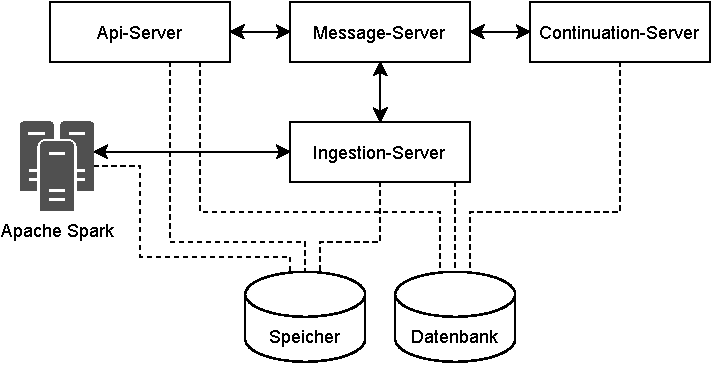
\includegraphics{Grafiken/Entwicklung-System-Architektur.pdf}
    \caption{Microservice-Architektur der Ingestion}
    \label{fig:system-architektur}
\end{figure}

\section{Plugins}

In \ref{ANF_04} wird durch ANF\_04 gefordert, dass zusätzlicher Code bei der Ingestion ausgeführt werden können soll.
Das soll durch Plugins umgesetzt werden.
Die Plugins werden jeder Datenquelle einzeln hinzugefügt und werden an verschiedenen, fest definierten Punkten der Ingestion ausgeführt. 
Da die Plugins eventuell auf Software-Bibliotheken zurückgreifen müssen, die nicht auf dem Data-Lake-System vorhanden sind, kann zusätzlich eine Liste von Abhängigkeiten der Plugins angegeben werden.

Bei der Ingestion gibt es zwei Stellen, an denen das Einbringen eines Plugins sinnvoll sein kann.
Die erste ist zum Laden der Daten als Load-Plugin.
Hier wird das standardmäßige Vorgehen der Ingestion mit dem des Plugins ersetzt.
Dadurch wird es möglich anders als nur über \textit{Apache Spark} Daten zu laden.
Ein Beispiel dafür ist die Verwendung einer REST-API als Datenquelle.
Das Plugin kann erst über mehrere Abfragen der REST-API den Datensatz abholen und diesen dann erst in eine DataFrame umwandeln.
Ein Load-Plugin muss immer eine DataFrame zurück geben, mit dem danach in der Ingestion weiter verfahren werden kann.
Damit ein DataFrame erstellt werden kann,  muss dem Plugin außerdem die entsprechende SparkSession mitgegeben werden.

Das After-Load-Plugin setzt im Gegensatz direkt nach dem Laden der Daten an.
Diesem Plugin wird das geladene DataFrame übergeben und es muss auch wieder ein DataFrame zurück geben.
Es kann genutzt werden um vor dem Speichern der Daten kleinere Anpassungen am Datensatz zu machen.
\section{Metadatenmodell}

Wie bereits erwähnt muss ein Modell erstellt werden, dass die Metadaten abbildet, die bei einer Ingestion erfasst werden (\cref{fig:datenmodell}).
Zu diesen Metadaten gehören alle Informationen über die Herkunft der Daten, also die Datenquelle und das Speicherziel.
Diese werden zum Großteil in für Spark erforderlichen Parametern widergespiegelt.
Ein weiterer Teil der Metadaten sind alle Informationen über die Ausführung einer Ingestion.

\subsection{DatasourceDefinition}

Das Metadatenmodell beschreibt eine Datenquelle und hat als zentrales Element das Konzept DatasourceDefinition.
Ein Teil des Modells besteht aus Feldern, die für Spark erforderlichen Informationen enthalten.
Dazu gehören: \begin{itemize}
    \item zusätzliche Abhängigkeiten für Spark (spark.jars.packages),
    \item das Format und Optionen für die Reader und
    \item bei benutzerdefinierten Speichersystemen das Format, die Optionen und einen Schreibmodus für die Writer.
\end{itemize}
Neben den Spark spezifischen werden noch folgende weitere Informationen erfasst: \begin{itemize}
    \item ein Name für die Datenquelle,
    \item die Id einer anderen Datenquelle, falls die aktuelle eine Update-Quelle ist,
    \item das Datum der Erstellung und letzten Änderung,
    \item den Namen der Id-Spalte in den Daten (wird später für die Deltaberechnung benötigt),
    \item den Typ, der zu lesenden Daten,
    \item eine Liste der zu laden Dateien, wenn es sich um eine Datei-Ingestion handelt,
    \item den Typ, wie die Daten geschrieben werden müssen,
    \item eine Liste mit der Zeitsteuerung für eine kontinuierliche Ingestion,
    \item eine Liste mit Plugindateien und
    \item eine Liste mit Abhängigkeiten der Plugins.
\end{itemize}

Die möglichen Lese-Typen ergeben sich aus der Betrachtung, wie die Daten in das Data-Lake-System gelangen und welche Struktur sie haben.
Bei einer Pull-Ingestion ist das System dafür verantwortlich Daten aus einer Quelle zu laden.
Dies ist zum Beispiel bei Datenbanken der Fall.
Das Gegenteil dazu ist eine Push-Ingestion, bei der die Daten direkt an den Data Lake gesendet werden.
Diese muss jedoch nochmal in zwei unterschiedliche Typen unterteilt werden.
Bei einer Stream-Ingestion, also bei Datenströmen, werden kontinuierlich neue Daten an das System gesendet.
Und bei einer File-Ingestion werden Dateien hochgeladen, die die Daten enthalten, wobei wichtig ist, dass alle Dateien das gleiche Dateiformat und je nach Typ eine ähnliche oder gleiche Struktur haben.
Die Dateien können sich in Daten- und Quelldateien unterscheiden.
Datendateien enthalten unstrukturierte Daten und werden einfach im HDFS mit abgelegt, ohne weiter verarbeitet zu werden.
Das könnten zum Beispiel Bilder oder Videos sein.
Quelldateien enthalten mindestens semistrukturierte Daten und dienen dem Zweck, in ein anderes Speicherformat, wie zum Beispiel Parquet oder eine Delta-Tabelle geschrieben zu werden.
Es ist nicht möglich, Daten direkt an die API zu senden.
Alle Push-Ingestions sollen über diese beiden Typen abgebildet werden.

Die möglichen Schreib-Typen werden aus den Speicherzielen abgeleitet.
Custom bedeutet, dass der in der DatasourceDefinition konfigurierte Speicher verwendet werden soll.
Delta ist das Speichern im internen Speicher aber mit einer Versionierung und Default ist das Speichern ohne Versionierung.

Für die Umsetzung einer unkomplizierten Versionierung der DatasourceDefinition werden alle veränderlichen Informationen in Revisionen gespeichert.
Das betrifft alle oben genannten Felder.
Die Revisionen einer DatasourceDefinition erhalten eine fortlaufende Nummer.
Die DatasourceDefinition selbst hält dann nur noch eine Liste aller Revisionen und die Nummer der aktuellen.

\subsection{IngestionEvent}

Das Modell für den Ablauf einer Ingestion ist das IngestionEvent.
Dieses enthält, wie die Revision, eine fortlaufende Nummer, ein Start- und Enddatum, den aktuellen Status indem es sich befindet, die Nummer der Revision mit der es gestartet wurde und eine Fehlernachricht, falls ein Fehler aufgetreten ist.

Das IngestionEvent kann auch zur DatasourceDefinition hinzugefügt werden.
Dafür werden Felder hinzugefügt, die alle IngestionEvents, die Nummer des letzten und die Nummer des letzten erfolgreichen IngestionEvents enthalten.

\begin{figure}
    \centering
    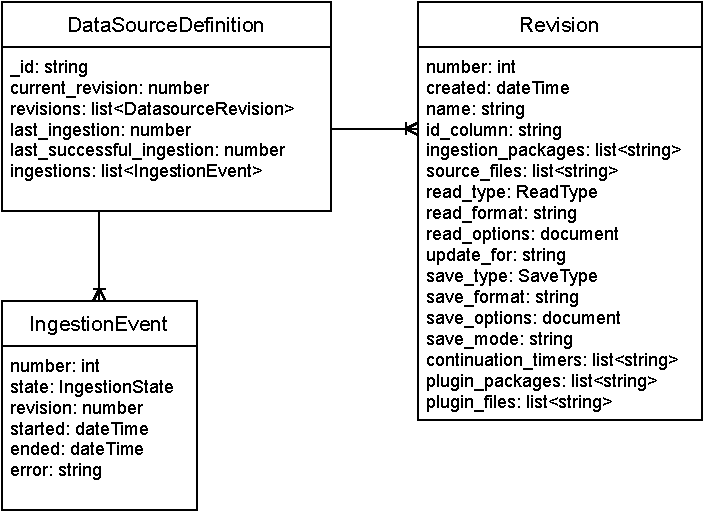
\includegraphics{Grafiken/Entwicklung-Datenmodell.pdf}
    \caption{Übersicht Metadatenmodell}
    \label{fig:datenmodell}
\end{figure}
\section{API-Service}

Für den API-Service müssen Endpunkte definiert werden.
Diese Endpunkte bilden die verschiedenen Funktionen ab, die auf der Ingestion-Schnittstelle ausgeführt werden können.
Dazu gehören die Verwaltung von Datenquellen und das Starten einer Ingestion.
Da es bereits festgelegt wurde, dass es sich um eine REST-Schnittstelle handelt, werden Endpunkte durch einen Pfad und eine HTTP-Methode definiert.
Nachfolgend werden alle Endpunkte aufgelistet.

\begin{table}[ht]
  \centering
  \begin{tabularx}{\linewidth}{lX}
    GET & /datasources \\
    \multicolumn{2}{l}{Liefert alle im System gespeicherten Datenquellen} \\
    \\
    GET & /datasources/\textless id\textgreater \\
    \multicolumn{2}{l}{Liefert die Datenquelle mit der im Pfad übergebenen Id} \\
    \\
    POST & /datasources \\
    \multicolumn{2}{l}{Bearbeitet die Daten Datenquelle mit der im Pfad übergebenen Id} \\
    \\
    PUT &  /datasources/\textless id\textgreater \\
    \multicolumn{2}{l}{Erstellt eine neue Datenquelle} \\
    \\
    GET &  /datasources/\textless id\textgreater/run \\
    \multicolumn{2}{l}{Startet eine Ingestion der Datenquelle mit der im Pfad übergebenen Id}
    
    
    
    %\hline
    %Pfad                                      & HTTP-Methode & Beschreibung                                                          \\
    %\hline \hline
    %/datasources                              & GET          & Liefert alle im System gespeicherten Datenquellen                     \\
    %\hline
    %/datasources/\textless id\textgreater     & GET          & Liefert die Datenquelle mit der im Pfad übergebenen Id                \\
    %\hline
    %/datasources                              & POST         & Erstellt eine neue Datenquelle                                        \\
    %\hline
    %/datasources/\textless id\textgreater     & PUT          & Bearbeitet die Daten Datenquelle mit der im Pfad übergebenen Id       \\
    %\hline
    %/datasources/\textless id\textgreater/run & GET          & Startet eine Ingestion der Datenquelle mit der im Pfad übergebenen Id \\
    %\hline
  \end{tabularx}
  %\caption{Endpunkte des API-Servers}
  \label{tab:enpoints}
\end{table}

Außerdem kümmert sich der API-Service um die Erstellung von Datenquellen, deren Revisionen und Ingestion-Events.
Bei Anfragen zum Starten einer Ingestion versendet der API-Server eine Nachricht, mit der Id der Datenquelle.
\section{Continuation-Service}

Für die Sicherstellung der korrekten Ausführung kontinuierlicher Ingestions, müssen regelmäßig alle Datenquellen überprüft werden.
Dabei gibt es zwei Bedingungen nach denen entscheiden wird, ob eine Ingestion werden muss.
Bei Datenströmen gilt allgemein, wenn dieser nicht läuft, dann muss die Ingestion automatisch neu gestartet werden.
Eine Ausnahme dabei ist, wenn die Verarbeitung durch den Benutzer explizit beendet wurde.

Der zweite Fall ist die Zeitsteuerung.
Für eine zeitgesteuerte kontinuierliche Ingestion werden einer Datenquelle ein oder mehrere Timer hinzugefügt.
Der Continuation-Service prüft, ob der Timer zu diesem Zeitpunkt zutrifft oder nicht.
Wenn das der Fall ist und bisher keine Ingestion auf der Datenquelle läuft, dann wird eine neue gestartet.

In Unix-Systemen gibt es bereits eine Lösung für die Notation solcher Timer.
Dort gibt es die sogenannten Cron-Jobs, mit deren Hilfe Aufgaben automatisch und regelmäßig ausgeführt werden können.
Dabei wird der Zeitpunkt der Ausführung über fünf Felder festgelegt.
Diese geben die Minute, die Stunde, den Tag des Monats, den Monat und den Tag der Woche als Zahlen an.
Als Erweiterung kann man "`*"' als Platzhalter für alle möglichen Werte verwenden, man kann mehrere Werte als mit Kommata getrennt angeben oder mit "`/x"' eine Liste in Schritten der Größe $x$ erzeugen \parencite{cron}.

Diese Notation soll auch für die Zeitsteuerung der Ingestions genutzt werden.
Als Referenz wird dabei die koordinierte Weltzeit (UTC) genommen, damit die Ausführung unabhängig vom Standort einheitlich bleibt.
Wenn eine Datenquelle mehrere Timer hat, reicht es aus, dass einer von diesen zutrifft.
\section{Ingestion-Service}
\label{sec:entw-ingestion}

Der Ingestion-Service hat die Aufgabe den Spark-Job für die Ausführung einer Ingestion zu erstellen, zu starten, zu überwachen und den Status des IngestionEvents anzupassen.
Dazu gehört das Festlegen des Ablaufs zum Laden der Daten in ein DataFrame, zur Deltaberechnung und zum Speichern.
Ein zweiter wichtiger Teil ist die Integration der Plugins in den Ingestion-Prozess.
Ebenfalls koordiniert der Ingestion-Service die parallele Ausführung von Ingestions.

Der Ingestion-Service wartet auf die Nachricht zur Ausführung einer Ingestion, mit der Id der DatasourceDefinition.
Als erstes wird geprüft, ob bereits eine Ingestion der Datenquelle aktiv ist.
Falls das nicht der Fall ist, wird ein neuer Prozess gestartet, indem die Ingestion ausgeführt wird.
Auf diese Art wird die Parallelität ermöglicht.

Der Ablauf einer Ingestion kann unabhängig vom Lese- und Schreib-Typ in einem allgemeinen Ablauf, wie in \cref{fig:ingestion-ablauf}, abgebildet werden.
Als erstes wird die Ingestion vorbereitet.
Hier werden die Plugins und deren Abhängigkeiten installiert und eine SparkSession erstellt.
Im nächsten Schritt werden die Daten aus der Quelle geladen.
Wenn es sich dabei um Änderungsdaten aus einer Update-Quelle handelt, können diese direkt in den entsprechenden Zieldatensatz eingepflegt werden.
Ist das nicht der Fall, folgt eine Entscheidung, ob Änderungsdaten berechnet werden müssen.
Es gelten die folgenden zwei Regeln: \begin{itemize}
    \item der Speicher-Typ ist Delta und
    \item es ist nicht die erste Ingestion dieser Datenquelle.
\end{itemize}
Wurden Änderungsdaten berechnet, werden diese eingepflegt.
Wurden keine berechnet, werden die Daten einfach gespeichert.
Ist das Speicherziel dabei ein Delta-Tabelle wird diese angelegt und ist es eine Parquet-Datei, dann werden die aktuellen Daten überschrieben.
Handelt es sich nicht um einen benutzerdefinierten Speicher, werden die alten Daten mit den neuen überschrieben.

\begin{figure}
    \centering
    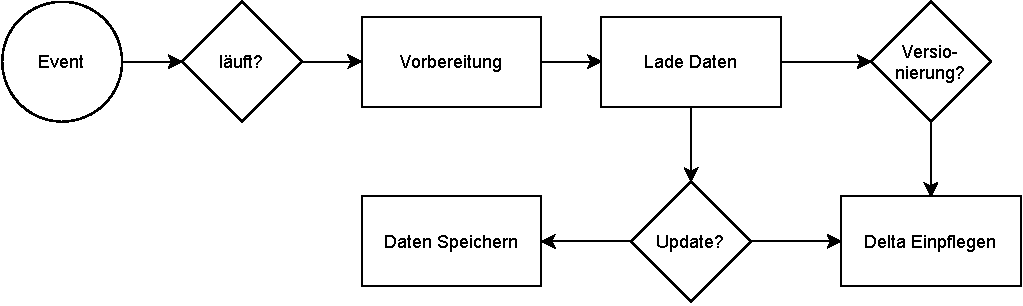
\includegraphics[width=\textwidth]{Grafiken/Entwicklung-Ingestion-Ablauf.pdf}
    \caption{Ablauf einer Ingestion}
    \label{fig:ingestion-ablauf}
\end{figure}
\chapter{Umsetzung}

Für eine Umsetzung der entwickelten Architektur ist zuerst die Frage der Techniken zu klären.
Dazu zählen die verwendete Programmiersprache, Frameworks und fertige Software.

\section{Nachrichtensystem}

Für die Übermittlung von Nachrichten zwischen verschiedenen Anwendungen gibt es sogenannte Message-Broker.
Diese koordinieren als Mittelsmann die Verteilung der Nachrichten an verschiedene Empfänger.
Das hat den Vorteil, dass der Sender unabhängig von den Empfängern wird und die Kommunikation asynchron statt finden kann \parencite{message-broker}.

Es gibt mittlerweile einige Projekte, diese Aufgabe auf verschiedene Arten lösen.
Hier wird dafür Apache Kafka verwendet, welches im Big Data Bereich weit verbreitet ist um Datenströme zu verarbeiten.
Daher macht es Sinn, dieses in das Data-Lake-System zu integrieren und darin bereit zu stellen.
Um das System dabei nicht unnötig komplex und zu groß werden zu lassen, wird daher auf einen anderen Message-Broker verzichtet.

Da Kafka ein Event-Streaming-System ist, wird ab hier nicht mehr vom Austausch von Nachtrichten, sondern von Events gesprochen.
Für diese Events müssen Topics zur Einordnung fetsgelegt werden.
Die Schlüssel sollten dabei so gewählt werden, dass Kafka auch für andere Datenströme verwendet werden kann, ohne, dass zu Konflikten kommt.
Daher werden die Topics der internen Kommunikation des Data-Lake-Systems immer mit "`dls\_\_"' als Prefix benannt werden.
Danach folgt der Bereich, den das Event betrifft, hier zum Beispiel "`ingestion"'.
An diesen Namen kann dann noch weiter Unterscheidung angehängt werden.
Für das Ausführen einer Ingestion wäre damit die Topic "`dls\_\_ingestion\_\_run"'.

Wenn mehrere Consumer in einer Gruppe für eine Topic sind, werden Events nicht an alle sondern immer nur an einen aus der Gruppe gesendet.
Dieser Mechanismus kann für den Lastausgleich an bestimmten Stellen verwendet werden.
Für die Ingestion kann so der Ingestion-Services einfach repliziert werden.
\section{Datenbank und Datenmodell}

Da das Datenmodell einer Datenquelle eine verschachtelte Struktur hat, bietet sich hier als einfachste Lösung die Verwendung einer Dokumenten-orientierten NoSQl-Datenbank an.
Das hat den Vorteil, dass diese Listen direkt in den Objekten der Datenquellen abgelegt werden können.
In relationalen Datenbanken, die Tabellen verwenden, müsste man für jedes Modell eine eigene Tabelle erstellen und die Verknüpfungen über über JOIN-Operationen auflösen.
Bei jeder Abfrage einer Datenquelle werden die verknüpften Einträge der Ingestion-Events oder Revisionen gebraucht, was somit zu einem größeren Aufwand führt.
Außerdem gibt es viele Anfragen auf die Datenquellen, da diese nicht zwischen den Mircoservices ausgetauscht werden und so nicht im Speicher vom Service verwaltet werden können.
Daher ist es effizienter die relevanten Daten direkt mit einer Abfrage laden zu können.
Hier kommt MongoDB\footnote{https://www.mongodb.com/} als Datenbank zum Einsatz.
MongoDB kann frei verwendet werden und bei bei größeren Datenmengen verteilt eingesetzt werden.

\section{Datenspeicher}

Für das Speichern von Daten mit einer Versionierung ist Delta Lake eine gut gepflegte und in Spark integrierte Lösung.
Neben den versionierten müssen auch Daten mit und ohne Struktur gespeichert werden.
Für strukturierte und semistrukturierte Daten kommt das Parquet-Format zum Einsatz.
Unstrukturierte Daten werden im ursprünglichen Format im HDFS abgelegt.

Als Speicher wird das HDFS verwendet.
In diesem können sowohl die Delta Tabellen als auch andere Parquet-, Quell- und Plugin-Dateien abgelegt werden.
Alle Microservices haben über die WebHDFS-Schnittstelle Zugriff auf die Daten.
Im HDFS wird eine Verzeichnisstruktur (\cref{fig:hdfs-folder}) für alle Daten des Data Lakes angelegt.
Diese geht von dem Ordner "`datalake"' aus, der im Root-Verzeichnis des HDFS angelegt wird.
In diesem Ordner werden die Unterordner
\begin{itemize}
    \item "`sources"' für Quell-Dateien,
    \item "`plugins"' für Plugin-Dateien und
    \item "`data"' für die Ablage von geladenen Daten erstellt.
\end{itemize}

In den Ordnern "`sources"' und "`plugins"' werden dann für jede Datenquelle Ordner mit deren Id angelegt, in denen die hochgeladenen Dateien abgelegt werden.

Für die geladenen Daten werden die Ordner \begin{itemize}
    \item "`structured"' für semi-/strukturierte Daten ohne Versionierung,
    \item "`unstructured"' für unstrukturierte Daten und 
    \item "`delta"' für semi-/strukturierte Daten mit Versionierung.
\end{itemize}
innerhalb des Ordners "`data"' angelegt.
Diese unterteilen sich dann ebenfalls wieder in Ordner für jede Datenquelle mit der Id als Name.

\begin{figure}
    \centering
    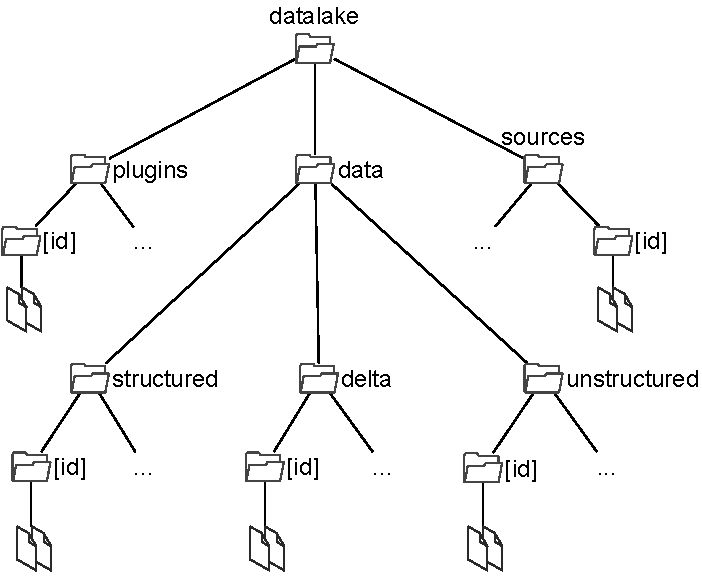
\includegraphics[width=.6\textwidth]{Grafiken/Umsetzung-Verzeichnisse.pdf}
    \caption{HDFS Verzeichnisstruktur}
    \label{fig:hdfs-folder}
\end{figure}
\section{API-Service}

Bei HTTP-Anfragen können Inhalte in der Anfrage als verschiedene Typen übergeben werden.
Hier wird der Typ \verb|mutltipart/forma-data| verwendet.
Bei diesem Typ können sowohl Text als auch Dateien übertragen werden.
Jeder Text oder jede Datei werden dabei als Wert betrachtet und müssen einen Schlüssel vergeben bekommen.
Das heißt, dass alle Informationen als Schlüssel-Wert-Paar an den API-Service gesendet werden.
Die Schlüssel, die verwendet werden sollen, werden wie folgt vergeben.
Die DatasourceDefinition bekommt den Schlüssel "`datasource-definition"'.
Der Wert dahinter kann entweder eine JSON-Datei oder ein JSON-Text sein.
Die Schlüssel der hochgeladenen Dateien sind frei wählbar.

Die DatasourceDefinition besteht zu Teilen aus Feldern, die automatisch durch die Services gefüllt werden.
Daher wird ein weiteres Datenmodell für die Eingabe von Informationen bei der REST-API benötigt.
Dafür wird die DatasourceDefinitionInput (\cref{fig:datasource-definition-input}) verwendet.
In diesem Modell befinden sich alle Felder, die durch den Benutzer befüllt werden können.
Aus den Daten dieses Modells erstellt der API-Service dann die Revisionen für die DatasourceDefinition.

\begin{figure}
    \centering
    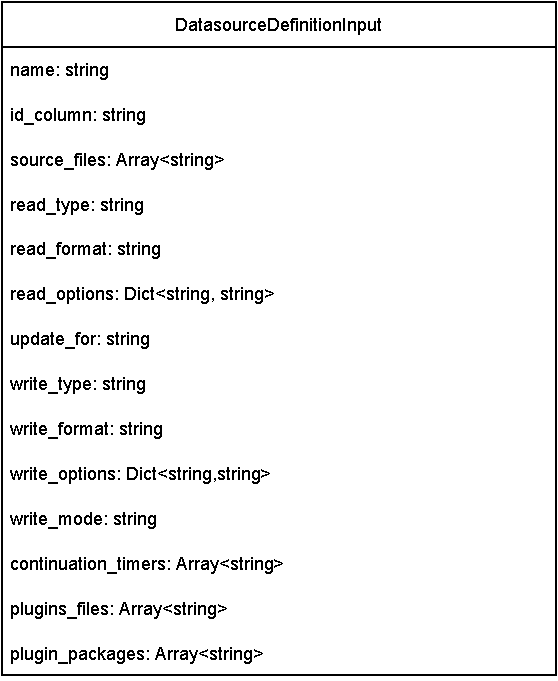
\includegraphics[width=.65\textwidth]{Grafiken/Umsetzung-Definition-Input.pdf}
    \caption{Felder Datenquellen-Eingabe}
    \label{fig:datasource-definition-input}
\end{figure}

\subsection{Hochladen von Dateien}

Für jede Datenquelle können Quell- oder Plugin-Dateien hochgeladen werden.
Um eine hochgeladene Datei in der Datenquelle auch zu verwenden, muss der Schlüssel, unter dem die Datei hochgeladen wird, in der entsprechenden Liste entweder unter "`source\_files"' oder unter "`plugin\_files"' hinzugefügt werden.
Alternativ können auch die Namen unter denen bereits Dateien für die Datenquelle gespeichert wurden in die Listen eingefügt werden.

Bei der Verarbeitung der Eingabe prüft der API-Service für jeden Eintrag der Listen, ob eine Datei mit diesem Schlüssel hochgeladen wurde.
Ist das der Fall, wird die entsprechende Datei in das HDFS hochgeladen.
Der Name, unter dem die Datei gespeichert wird, setzt sich aus der Nummer der Revision, dem vergebenen Schlüssel und der Endung der Datei zusammen.
Lädt man also eine bei der ersten Erstellung einer DatasourceDefinition eine Datei "`data.json"' mit den Schlüssel "`file"' hoch, wird diese als "`r000\_file.json"' im "`sources"'-Ordner der DarasourceDefinition gespeichert.
Analog werden Plugin-Dateien genauso behandelt.

Wenn keine Datei in der Anfrage gefunden wurde, wird geschaut, ob im HDFS eine Datei mit dem Namen existiert.
Wird eine Datei gefunden, wird der Name an die neue Revision angehangen.
Es ist wichtig zu beachten, dass alle Dateien der alten Revision, die nicht explizit in einer der Listen angegeben werden, nicht in der neuen Revision verwendet werden.
Sie bleiben jedoch gespeichert und können später wieder hinzugefügt werden.
Da die Dateien nach den Datenquellen aufgeteilt sind, ist es aktuell nicht möglich Plugins oder Quell-Dateien in anderen Datenquellen wieder zu verwenden.
Hier müsste man die Datei für jede Datenquelle hochladen.

\section{Continuation-Service}

Der Continuation-Service führt durchgehend eine Schleife zum Überprüfen der Datenquellen aus.
Bei der Prüfung wird immer der Status des aktuellsten IngestionEvent betrachtet.
Je nach Datenquelle wird dann entschieden, ob eine Ingestion gestartet werden soll.
Die Logik der Schleife besteht aus drei Teilen, wovon zwei die Datenquellen prüfen und einer die Zeit steuert, nachdem die Schleife erneut ausgeführt wird (\cref{algo:ci-loop}).
Das soll nur maximal jede Minute geschehen, da auch keine schnellere Ausführung über die Timer definiert werden kann.

Im ersten Teil werden alle Datenquellen einer Datenstrom-Ingestion kontrolliert.
Für diese wird eine neue Ingestion gestartet, wenn der Status "`FINISHED"' ist.
Der Status "`STOPPED"' bedeutet, dass die Ausführung mit Absicht beendet wurde und manuell gestartet werden muss.

Der zweite Teil überprüft alle Datenquellen, bei denen ein oder mehrere Timer gesetzt wurden.
Wenn der Status des letzten IngestionEvents nicht "`STOPPED"' oder "`FINISHED"' ist, wird die Überprüfung dieser Quelle abgebrochen.
Ansonsten wird jeder Timer mit dem aktuellen Zeitpunkt verglichen.
Hier wird die Methode $is_now$ verwendet.
Sie wird durch eine Python-Bibliothek bereitgestellt und prüft ob ein Cron-Timer, die auch für die kontinuierliche Ingestion eingesetzt werden, zum aktuellen Zeitpunkt zutrifft.
Trifft der Timer zu, wird eine Ingestion für die Datenquelle gestartet und sofort die nächste Datenquelle überprüft.

Der dritte Teil kontrolliert die Ausführungshäufigkeit.
Dazu wird am Anfang der Schleife der Startzeitpunkt gespeichert.
Nachdem alle Überprüfungen beendet wurden, wird auch der Endzeitpunkt gespeichert.
Wenn die Differenz der beiden geringer ist als eine Minute, wird die Schleife für die Dauer der Differenz angehalten.
Damit ist sichergestellt, das sie nicht häufiger als einmal pro Minute ausgeführt wird.

\begin{algorithm}
    \caption{Continuation loop}
    \label{algo:ci-loop}
    
    \KwData{-}
    \KwResult{-}
    
    $loopStart \gets$ current\_time() \;
    
    $streams \gets$ all\_datasource\_definition\_of\_type\_stream() \;
    \ForAll {$definition$ in $streams$} {
        $event \gets definition.last\_ingestion$ \;
        \If {$event.state$ is FINISHED} {
            publish\_run\_event\_for($definition.id$) \;
        }
    }
    
    $timed \gets$ all\_datasource\_definitions\_with\_timers() \;
    \ForAll {$definition$ in $timed$} {
        $event \gets definition.last\_ingestion$ \;
        $timers \gets definition.revision.continuation\_timers$  \;
        \If {$event.state$ is STOPPED or FINISHED} {
            \ForAll {$timer$ in $timers$} {
                \If {is\_now($timer$)} {
                    publish\_run\_event\_for($definition.id$) \;
                    \textbf{break}
                }
            }
        }
    }

    $loopEnd \gets$ current\_time() \;
    $loopDuration \gets loopEnd - loopStart$ \;
    \If {$loopDuration < 60$} {
        sleep($60 - loopDuration$) \;
    }

\end{algorithm}


\section{Ingestion-Service}

Wie in \fref{sec:entw-ingestion} beschrieben, wird für ein Event ein Prozess gestartet.
Der Name der Topic des Events zum Starten einer Ingestion ist "`dls\_\_ingestion\_\_run"'.
In \fref{sec:ingestion-run} wird der detailliere Ablauf mit den verschiedenen Wegen für Read- und SaveTypes beschrieben.
Vorher werden die benötigt Grundlagen zur Ausführung erläutert.

\subsection{Berechnen und Speichern der Änderungsdaten}
Um Änderungen in eine Delta Tabelle zu übernehmen, müssen die Änderungsdaten in einem Format sein, dass Aufschluss darüber gibt, welche Daten hinzugefügt, welche geändert und welche gelöscht worden sind.
Das hier verwendete Format muss genau dem gleichen Schema entsprechen, wie die original Daten.
Zusätzlich soll eine Spalte oder ein Feld auf der obersten Eben mit dem Namen "`cd\_deleted"' vorhanden sein.
Es enthält einen Boolean-Wert, der sagt, ob der Eintrag aus den Daten gelöscht wurde oder nicht.
Der Datensatz mit den Änderungsdaten darf außerdem nur geänderte Daten enthalten.
Aus diesem Format können, wie später gezeigt, die drei Operationen abgeleitet werden.

Um nicht auf ein externes Change-Data-Capture-System angewiesen zu sein, gibt es eine interne Lösung, die auf alle (semi-)strukturierten Daten angewendet werden kann.
Der \cref{algo:delta-calc} zeigt, wie aus zwei DataFrames die Änderungsdaten erzeugt werden.
Als Eingabe werden ein linkes DataFrame, mit dem aktuellen internen Stand, eine rechtes DataFrame, mit den neuen Daten und der Name der Id-Spalte benötigt.
Das Ergebnis ist ein DataFrame mit allen aktualisierten Datensätzen.
Es hat das gleiche Schema wie die Ursprungsdaten, aber mit der zusätzlichen Spalte, die Auskunft darüber gibt, ob ein Datensatz gelöscht wurde.

\begin{algorithm}
    \caption{Deltaberechnung}
    \label{algo:delta-calc}
    \KwData{leftDataFrame, rightDataFrame, idColumn}
    \KwResult{changeDataFrame}
    $leftDataFrame \gets$ add column with row hash \;
    $leftDataFrame \gets$ prefix column names with "`left\_"' \;
    $rightDataFrame \gets$ add column with row hash \;
    $rightDataFrame \gets$ prefix columnnames with "`right\_"' \;

    $changeDataFrame \gets$ full join over $idColumn$ of $leftDataFrame$ and $rightDataFrame$ \;

    $changeDataFrame \gets$ remove all rows where $left\_hash$ equals $right\_hash$ \;

    $changeDataFrame \gets$ remove hash columns

    $changeDataFrame \gets$ add row $cd\_deleted$ \;
    \eIf{$right\_idColumn$ is $null$}{$cd\_deleted = true$}{$cd\_deleted = false$}

    $changeDataFrame \gets$ merge left and right $idColumn$ into one $idColumn$
    \eIf{$left\_idColumn$ is not $null$}{$idColumn = left\_idColumn$}{$idColun = right\_idColumn$}

    $changeDataFrame \gets$ merge remaining columns with left and right value by always taking the right and removing prefix

\end{algorithm}

Das Einpflegen der Änderungen wird über die Delta Lake API gelöst.
Dazu werden die Änderungsdaten mit den aktuellen Daten über die Id-Spalte zusammengeführt.
Dabei können verschieden Fälle definiert werden.
Wenn die Ids einer Zeile gleich sind und die Spalte "`cd\_deleted"' $true$ enthält, wird die Zeile aus den Daten gelöscht, ansonsten wird der Datensatz aktualisiert.
Wenn die Ids nicht übereinstimmen und die Spalte "`cd\_deleted'" $false$ ist, dir der Datensatz als neue Zeile eingefügt.

\subsection{Plugins verwalten}
Für jede Ingestion wird auf dem Speichersystem des Mircoservices ein temporärer Ordner angelegt, in den die Plugins und deren Abhängigkeiten installiert werden.
Nach der Installation wird noch eine Datei angelegt, die für alle Pakete die Versionen enthält.
Das dient dazu, bei einer erneuten Ausführung auf dem Service nicht alle Pakete neu installieren zu müssen, sondern nur die mit geänderten Version.
Das beschleunigt die Ausführung der Ingestion.
Zum Schluss wird der Ordner, in den die Pakete installiert wurden an den Python-Pfad mit angehangen.
Damit wird dieser während der Ausführung manipuliert und die Pakete sind verfügbar.
Da jede Ingestion in einem eigenen Prozess beeinflussen die Änderungen an dem Python-Pfad den Ingestion-Service oder andere Prozesse nicht.

Im zweiten Schritt wird jede Python-Datei im Pluginordner als Modul geladen.
Die im Modul verfügbaren Methoden werden dann überprüft, ob sie auf eine Definition der möglichen Plugins passen.
Dazu wird der \fref{algo:check-method} verwendet.
Diesem werden das geladene Modul, ein Name der Methode, ein optionaler Rückgabetyp der Methode und eine Liste von Parameter, bei denen Name und Typ definiert ist.
Zur Überprüfung können alle Methoden in dem Modul auf ihren Namen geprüft werden.
Wenn eine Methode gefunden wurde, wird eine Signatur erzeugt und mit der übergebenen Definition verglichen.
Das Ergebnis sagt dann, ob diese Methode ein Plugin ist oder nicht.

Jedes geladene Modul wird auf Load- oder AfterLoad-Methoden geprüft.
Eine gefundene Load-Methode überschreibt immer die letzte gefunden, da bei einer Ausführung auch das Ergebnis dieser Methoden überschrieben werden würde.
Die AfterLoad-Methoden dagegen werden in einer Liste gespeichert.


\begin{algorithm}
    \caption{Pluginmethode überprüfen}
    \label{algo:check-method}

    \KwData{$plugin$, $name$, $return\_type$, $parameters$}

    \KwResult{$matches$}

    \If{plugin has NOT method with name $name$}{
        \Return{false}
    }

    $signature \gets$ signature of mehtod $name$

    \If{$return\_type$ is given AND $signature$ NOT returns type of $return\_type$}{
        \Return{false}
    }

    \ForAll{$param$ in $parameters$}{
        \If{$signature$ has NOT a parameter named $param.name$}{
            \Return{false}
        }

        \If{$signature$ type of parameter $param.name$ is NOT $parameter.type$}{
            \Return{false}
        }
    }

    \Return{true}

\end{algorithm}

\subsection{Ausführung der Ingestion}
\label{sec:ingestion-run}
Die Ausführung startet mit der Initialisierung, die die für die Ingestion benötigte Daten lädt.
Das ist zum Beispiel die DatasourceDefinition zu der Id aus den Events.
Danach wird entschieden ob eine Ingestion über Spark notwendig ist.
Hier spielt der Lesetyp eine große Rolle.
Eine Ingestion von Datendateien benötigt keine Spark, es werden einfach direkt die Dateien in das entsprechende Zielverzeichnis kopiert.
Für alle anderen Typen wird im nächsten Schritt die Ingestion vorbereitet.
Es werden die Plugins aus dem HDFS geladen und eine SparkSession erstellt.
Das Laden der Daten in ein DataFrame geschieht anschließend entweder über ein Plugin in oder das Standardvorgehen.
Falls auch After-Load-Plugins vorhanden sind werden diese ausgeführt.
Für die geladenen Daten wird dann entschieden, ob es sich um Änderungsdaten handelt oder welche berechnet werden müssen.
Je nach Schreib-Typ werden dann die Daten beziehungsweise Ändeurngsdaten gespeichert.
Für Datenströme wird am Ende noch ein Hintergrund Task gestartet, der auf Kafka Events zum stoppen dieser Ingestion wartet.
Hierfür wird die Topic "`dls\_\_ingestion\_\_stop\_ingestion"' mit der Id als Wert verwendet.
Wenn die Ingestion beendet wurde, wird zum Schluss die SparkSession gestoppt.

\begin{figure}
    \centering
    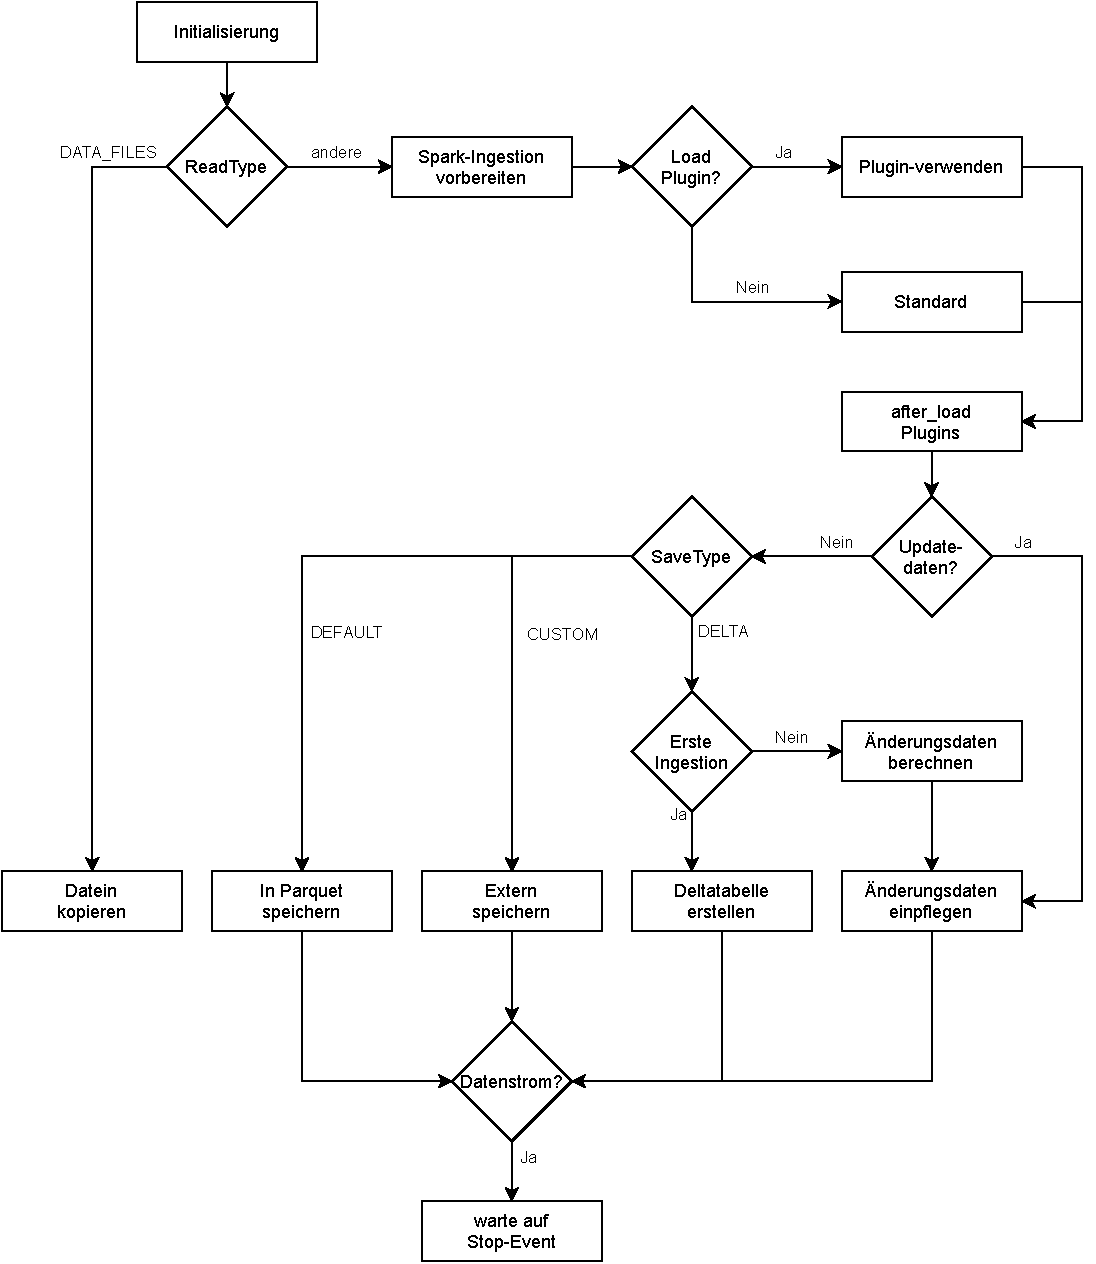
\includegraphics[width=\textwidth]{Grafiken/Umsetzung-Ingestion-Ablauf.pdf}
    \caption{Ablauf einer Ingestion}
    \label{fig:umsetz-ingestion-ablauf}
\end{figure}

\chapter{Evaluierung}
\chapter{Ausblick}

\newpage

\printbibliography

\end{document}
